\setcounter{step}{0}
%------------------------------------------
% information doc
\subsection{Cheesecake so slaným karamelom}
%------------------------------------------

\begin{ingredient}
%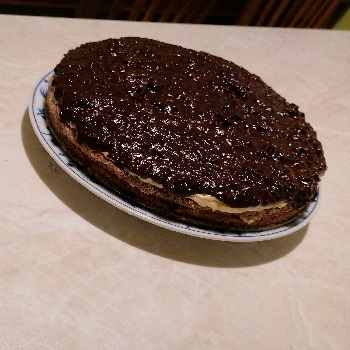
\includegraphics[height=5.5cm]{images/daim}
\def\portions{4}%
\textbf{{\normalsize Ingrediencie (\portions porcie):}}
%\vspace{0.5cm}
\begin{main}
	\item 
\end{main}
\begin{subingredient}{Cesto}
	\item 15g sušienky
	\item 80g maslo
\end{subingredient}
\begin{subingredient}{Plnka}
	\item 500g mascarpone
	\item 250g riccoty???/smotany??? salka???
	\item 3 vajíčka???
	\item 4PL cukor
\end{subingredient}
\begin{subingredient}{Slaný karamel}
	\item 1 cà.c de test1
	\item 1 à 2 cà.S de test2
	\item 3 gouttes de test3
	\item 8 morceaux de test4.	
\end{subingredient}

\end{ingredient}
\begin{recipe}
\textbf{{\normalsize Príprava:}}
\begin{enumerate}

\item{Maslové sušienky rozdrviť a primiešať maslo}
\item{Vystelieme formu na pečenie papierom a natlačíme na kraje sušienky s maslom}
\item{Dáme korpus piecť na 10-15 minút na 180° a zatiaľ zmiešame mascarpone s vajíčkami, cukrom, smotanou}	
\item{Zmesou naplníme korpus a dáme piecť na 40-50 minút}
\item{Pripravíme slaný karamel:}
\begin{enumerate}
\item{Skaramelizujeme cukor}
\item{Pridáme maslo}
\item{Prilejeme smotanu}
\item{Prídáme 1/2 lyžičky soli}
\end{enumerate}
\item{Polejeme, necháme v chladničke vychladnúť}

\end{enumerate}
\end{recipe}

\begin{notes}

\end{notes}
\clearpage	